% @ref:paper-methods
% Method: @link:doc-paper; @link:specification.
% Related: @link:paper-build-tables.
% @tag:methods
% SPDX-License-Identifier: MIT
% Copyright (c) 2026 John Larue
\documentclass[10pt]{article}
\usepackage[letterpaper,margin=1.05in]{geometry}
\usepackage{lmodern}
\usepackage[T1]{fontenc}
\usepackage{microtype,amsmath,amssymb,booktabs,longtable,array}
\usepackage{xcolor,tikz,pgfplots,float,flafter,placeins}
\usetikzlibrary{arrows.meta,positioning,calc,shapes.geometric}
\pgfplotsset{compat=1.18}
\definecolor{ink}{HTML}{1F2430}
\definecolor{mut}{HTML}{5B6675}
\definecolor{navy}{HTML}{27476E}
\definecolor{acc}{HTML}{3E6B9E}
\definecolor{amb}{HTML}{B45309}
\definecolor{grn}{HTML}{1F7A57}
\usepackage[colorlinks=true,citecolor=navy,urlcolor=navy,linkcolor=navy]{hyperref}
\usepackage{xurl}
% @ref:figure-style
% Method: @link:doc-paper.
% Related: @link:paper-methods.
% @tag:methods
% Vector figure language adapted from the companion egg paper.
\tikzset{
  >=Stealth,
  font=\footnotesize,
  fbox/.style={draw=ink!65, rounded corners=2.5pt, fill=white,
    align=center, inner sep=6pt, text=ink},
  flow/.style={->, thick, ink!75},
  planned/.style={fbox, dashed, draw=acc, fill=acc!5},
}
\pgfplotsset{score/.style={
  width=10.4cm, height=4.0cm, scale only axis,
  axis x line*=bottom, axis y line*=left,
  y axis line style={draw=none}, ytick style={draw=none},
  axis line style={ink!45}, tick style={ink!35},
  xmajorgrids=true, grid style={ink!10},
  y dir=reverse, ymin=-0.55,
  yticklabel style={font=\footnotesize, text=ink, align=right},
  xticklabel style={font=\scriptsize, text=mut},
  xlabel style={font=\footnotesize, text=mut},
  scaled x ticks=false, /pgf/number format/1000 sep={},
  /pgf/number format/fixed,
  clip=true,
}}
\newcommand{\scoreplot}[1]{%
  \addplot[only marks, mark=*, mark size=2.4pt, color=acc,
    mark options={fill=acc,draw=acc},
    error bars/.cd, x dir=both, x explicit,
    error bar style={line width=1.2pt}, error mark options={line width=0.9pt}]
    table[x=point, y=row, x error minus expr=\thisrow{point}-\thisrow{low},
      x error plus expr=\thisrow{high}-\thisrow{point}] {#1};
  \addplot[only marks, mark=diamond*, mark size=3pt, color=amb,
    mark options={fill=amb,draw=amb}]
    table[x=measured,y=row] {#1};
}
\newcommand{\scorelegend}{%
  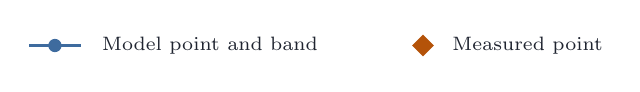
\begin{tikzpicture}[font=\scriptsize]
    \draw[acc, line width=1.2pt] (0,0)--(0.65,0);
    \fill[acc] (0.325,0) circle (2.4pt);
    \node[anchor=west,text=ink] at (0.8,0) {Model point and band};
    \node[diamond,fill=amb,inner sep=2pt] at (5,0) {};
    \node[anchor=west,text=ink] at (5.25,0) {Measured point};
  \end{tikzpicture}%
}

\hypersetup{pdftitle={Downstream: methods and validation},pdfauthor={John Larue}}
\setlength{\emergencystretch}{2em}
\makeatletter
\newcommand{\tableinput}[1]{\@@input #1 }
\makeatother
\input{generated/macros}
\title{A Citation-Calibrated Model of the\\Downstream Consequences of Worker Displacement}
\author{John Larue\\\small xh1b.org}
\date{October 2026\\\small Parameter set \ParameterVersion}
\begin{document}
\maketitle
\begin{abstract}
We present \texttt{downstream}, an open-source model that propagates
worker-displacement exposure through a ledger of published effects.
It distinguishes earnings gaps, direct effects, relative risks, and
jobs-per-job multipliers. Each parameter retains its citation, evidence
precision tier, population scope, and uncertainty band. Scenario counts
require verified baselines. Parameter sampling, exact moment calculations,
sensitivity analysis, and named structural variants expose uncertainty
in both estimates and composition choices. Current China-shock
retrodictions show mixed results: family-status contrasts are covered,
while mortality discrepancies and lower-quartile earnings underprediction
remain. Experimental extensions compare household earnings trajectories,
age-stratified mortality, and age-timed child earnings values, and propagate
documented baseline and declared exposure uncertainty separately.
Independent event back-tests remain blocked on data, and prospective
forecasts have not yet been registered. We report those limits alongside
the implemented methods. Outputs are conditional population-average
estimates, not predictions about individuals or proof that an exposure
was caused by a particular filing or employer. A current mathematical
review identifies mortality transport, baseline, and place-counterfactual
limits; numerical consistency alone does not
establish causal validity.
\end{abstract}

% @ref:paper-introduction
% Method: @link:doc-model-card; @link:doc-prior-attempts.
% @tag:methods
\section{Introduction}
Worker displacement has consequences beyond a worker's immediate earnings.
The underlying studies measure different outcomes in different populations:
worker earnings, mortality, and children's later earnings are prominent
examples \cite{jacobson1993,sullivan2009,oreopoulos2008}.
A combined model must state how those estimates can be used together.
A citation alone does not justify multiplication: a jobs-per-job multiplier
and an intergenerational earnings elasticity act on different quantities.

This model makes those distinctions explicit. It provides a typed ledger,
a versioned parameter set, reproducible uncertainty calculations, and
validation results that retain misses. Its present implementation is a
conditional propagation model with population aggregation, with a limited
annual household earnings prototype. It does not
simulate individual labor-market matching, migration, or behavioral
interactions. The term microsimulation describes the intended family-level
use; it should not imply that the code currently advances a representative
synthetic population through an annual life cycle.

% @ref:paper-related-work
% Method: @link:doc-prior-attempts; @link:doc-life-course-research-plan.
% @tag:methods
\section{Relation to other modeling approaches}
\subsection{Life-course and household microsimulation}
The intended person-and-place simulator belongs to an established research
tradition. SimPaths projects individual and household histories across
work, family relationships, health, and finances in an open-source
framework \cite{bronka2025simpaths}. It is a close architectural
reference for dynamic feedback and household context. LifeSim combines
developmental, economic, social, and health outcomes across an English
birth cohort's lifespan \cite{skarda2021lifesim}. It is especially relevant
to linking childhood circumstances with later outcomes. Neither project
should be reduced to a collection of isolated outcome multipliers.

Urban Institute's DYNASIM ages individuals and families through demographic
and economic transitions, including marriage, divorce, work, earnings,
disability, and retirement \cite{urban2015dynasim}. The Future Elderly
Model connects health and economic outcomes to evaluate alternative
health and policy scenarios \cite{uscFEM}. These programs provide useful
precedents for baseline trajectories, family structure, scenario analysis,
and empirical evaluation. Their domains and target populations differ;
this comparison is selective, not a systematic ranking of model quality.

Downstream currently has a narrower implementation: cited response
coefficients and count conversions conditional on an externally supplied
exposure. Its proposed contribution is an inspectable connection between
evidence applicability, composition restrictions, uncertainty, and
accessible scenario comparison. Openness, simulation of multiple domains,
and citation of evidence alone do not establish novelty. Whether its
composition rules improve out-of-sample performance remains a research
question, not a demonstrated advantage over these predecessors.

\subsection{Causal composition and population consequences}
Our design separates three tasks often combined in larger models:
estimating an exposure, propagating its consequences, and evaluating the
result. The exposure is supplied by the caller. The household prototype
reuses observed employment transitions under declared assumptions; a full
dynamic population model would additionally need entry, exit, and linked
demographic and economic transitions. An interacting-agent model would need
behavioral rules and a network; neither is present here.

Regional multipliers enter as a separate count boundary, following the
local-employment literature \cite{moretti2010}. They are not passed through
an earnings chain. Evidence synthesis enters through published individual
studies and meta-analyses \cite{paul2009,evans2008}. We compose selected
links under declared assumptions rather than pool unlike estimands into a
single effect. The model is therefore an auditable synthesis of conditional
responses, not a newly identified causal estimate of the entire system.

% @ref:paper-model
% Method: @link:specification; @link:doc-evidence-classification-0-4.
% Related: @link:figure-model.
% @tag:model
\section{Model and evidence}
Figure~\ref{fig:model} separates supplied inputs, model operations, and
reported outputs. Its arrows describe computation; they do not establish
that a causal pathway is identified.
% @ref:figure-model
% Method: @link:doc-causal-graph-plan.
% Implementation: @link:code-ledger.
% Related: @link:paper-model.
% @tag:model
\begin{figure}[t]
\centering
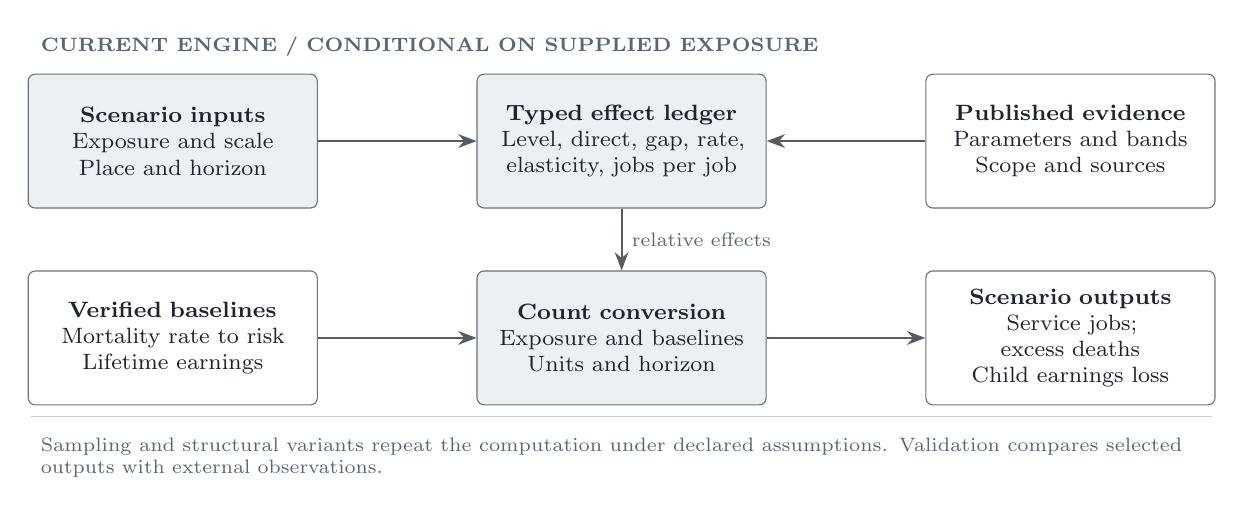
\begin{tikzpicture}
  \node[anchor=west,font=\scriptsize\bfseries,text=mut] at (0,1.0)
    {CURRENT ENGINE / CONDITIONAL ON SUPPLIED EXPOSURE};
  \node[fbox,fill=acc!10,text width=3.25cm,minimum height=1.7cm] (input) at (1.8,-0.2)
    {\textbf{Scenario inputs}\\Exposure and scale\\Place and horizon};
  \node[fbox,fill=acc!10,text width=3.25cm,minimum height=1.7cm] (ledger) at (7.5,-0.2)
    {\textbf{Typed effect ledger}\\Level, direct, gap, rate,\\elasticity, jobs per job};
  \node[fbox,text width=3.25cm,minimum height=1.7cm] (evidence) at (13.2,-0.2)
    {\textbf{Published evidence}\\Parameters and bands\\Scope and sources};
  \node[fbox,text width=3.25cm,minimum height=1.7cm] (baseline) at (1.8,-2.7)
    {\textbf{Verified baselines}\\Mortality rate to risk\\Lifetime earnings};
  \node[fbox,fill=acc!10,text width=3.25cm,minimum height=1.7cm] (convert) at (7.5,-2.7)
    {\textbf{Count conversion}\\Exposure and baselines\\Units and horizon};
  \node[fbox,text width=3.25cm,minimum height=1.7cm] (output) at (13.2,-2.7)
    {\textbf{Scenario outputs}\\Service jobs; excess deaths\\Child earnings loss};
  \draw[flow] (input)--(ledger);
  \draw[flow] (evidence)--(ledger);
  \draw[flow] (ledger)--(convert)
    node[midway,right,font=\scriptsize,text=mut] {relative effects};
  \draw[flow] (baseline)--(convert);
  \draw[flow] (convert)--(output);
  \draw[ink!25] (0,-3.7)--(15,-3.7);
  \node[anchor=north west,align=left,font=\scriptsize,text=mut,text width=14.5cm] at (0,-3.85)
    {Sampling and structural variants repeat the computation under declared assumptions.
     Validation compares selected outputs with external observations.};
\end{tikzpicture}
\caption{The current calculation boundary. Exposure is supplied, not inferred.
The ledger separates effect types before count conversion. A citation records
provenance; it does not by itself establish transportability or causal composition.}
\label{fig:model}
\end{figure}


% @ref:paper-exposure
% Method: @link:doc-exposure-semantics-0-4.
% Implementation: @link:code-scenario; @link:code-employer.
% Verification: @link:test-exposure-semantics.
% @tag:exposure
\subsection{Exposure and outcomes}
A scenario supplies displaced-worker exposure $N$, children per exposed
worker $C$, independently documented net tradable-job loss $T$, a job class, and a mortality window $Y$. The tradable-share field is metadata only; it does not infer $T$ from $N$.
The worker module reports earnings and mortality responses. The child
module reports earnings across three descendant generations. Family and
community modules expose additional pathways, but their availability in
a module does not imply that the scenario count interface reports them.
The current count interface returns local service jobs, excess deaths,
and child lifetime earnings losses, subject to verified baselines and
outcome-specific applicability checks. Default results are illustrative
reference calculations; a documented target population and reviewed
transport decision are required for headline eligibility.
The mortality count is a reference scenario for US men aged 45--54. Its
displacement effect comes from a study of high-seniority men. The child
earnings link comes from Canadian father--son firm closures and uses a US
male lifetime-earnings baseline in 2024 dollars. Applying either result to
a mixed or unknown population requires a separate transport argument.
Receiving-community crime links use source-specific population shares:
an undocumented-share percentage-point change for Light--Miller's
log-rate response, and a regular-resident share ratio for Bianchi's
log-log response. They are separate evidence inputs, not consequences
inferred from displaced-worker exposure. The named adapter retains
different source windows and fixed-effects versus IV roles. Bianchi's
calculation uses the available 2010 working-paper version; reconciliation
with the 2012 published article remains pending. Correct units do not
establish target transport. Optional incident differences
use the same supplied post population in both rate scenarios and concern
an annual endpoint, not cumulative crimes.

The entity adapter accepts either a documented exposure or a warehouse
aggregate with a stored total and components. The warehouse mapping checks
agreement between the headline and breakdown totals. It checks that the
worker-equivalent base, wage-depression, and applicable WARN components
reconcile within the upstream rounding tolerance. It preserves the total;
it does not re-estimate a wage-gap formula or add a notice count to a
worker count. Source and method references accompany the result. Person
subjects use the same population-average impact framing as employers.
This interface does not establish a causal link between filings and
worker displacement.

% @ref:paper-composition
% Method: @link:spec-composition.
% Implementation: @link:code-ledger; @link:code-units.
% Verification: @link:test-ledger.
% @tag:model
\subsection{Typed composition}
Let $v$ be a counterfactual-relative earnings level, with no loss represented
by $v=1$. Let $p$ be a parameter and $t$ an intergenerational transmission
coefficient. The ledger distinguishes
\begin{align}
 \text{level:}\quad &v'=vp,\\
 \text{direct:}\quad &v'=p,\\
 \text{gap:}\quad &v'=1-t(1-v).
\end{align}
A rate step records a relative effect for later conversion against a
baseline. A level ratio multiplies a count outside the chain. An
elasticity converts an input percentage change into an outcome percentage
change. These distinctions prevent a transmission coefficient from being
mistaken for a relative earnings level.

For the current parameter points, the direct child level is
\ChildPoint{}, the grandchild level is \GrandchildPoint{}, and the
 great-grandchild level is \GreatgrandchildPoint{}.
These values come from the same code used by the CLI; the first is the
direct child estimate and the later values propagate its gap
\cite{oreopoulos2008,solon1992,corak2013,chetty2014,lindahl2015,adermon2018}.
The father's earnings shock is not multiplied into the directly estimated
child effect. Repeated transmission beyond the identified generations
remains a modeling assumption.

Even the first transmission requires an extra causal assumption: a
between-family income association need not equal the response to a
displacement intervention. If $t$ is instead interpreted literally as
a constant log--log elasticity, the finite-change mapping is $v'=v^t$.
The implemented gap rule is its first-order expansion about $v=1$,
$v^t=1+t(v-1)+O((v-1)^2)$. Thus it is an explicit linear approximation,
not an exact conversion of a log elasticity. The implemented
\texttt{log\_elasticity\_transmission} ensemble variant compares the
finite-change mapping with the default gap rule using the same cited
coefficient. Both retain the structural-transmission label; neither is an
independently identified transmission of a displacement effect.

Parallel divorce and family-size pathways are not silently added to the
displacement pathway. The same affected children may appear in several
studies, and summation can double-count their losses. A named structural
variant exposes gap-additive composition as an experiment rather than
making it the default.

% @ref:paper-parameters
% Method: @link:doc-citing.
% Implementation: @link:code-params; @link:code-citations.
% Verification: @link:test-params.
% @tag:evidence
\subsection{Parameter custody}
This build contains \ParameterCount{} parameter rows in set
\ParameterVersion{}. Appendix~\ref{app:parameters} is generated directly
from the parameter file. Precision tiers describe how the number was
extracted: \texttt{EXACT} denotes a pinned table or full-text estimate;
abstract/results variants identify the narrower source read;
\texttt{canonical} marks an established value with remaining extraction
work. Precision of extraction is distinct from strength of causal
identification. Associational conversion factors and parallel evidence
must retain their limitations even when transcribed exactly.

Each row also stores population scope and notes on its band. Bands can
represent reported uncertainty, a range across specifications or studies,
or an explicitly declared approximation. They are not interchangeable
confidence intervals. The audit checks citation resolution, units, and
parameter structure. It cannot prove that a source has been interpreted
correctly. Full notes and evidence classes remain in the CSV and
bibliography rather than being replaced by the compact appendix.

% @ref:paper-counts
% Method: @link:doc-mortality-source-reconciliation-2026-09-10; @link:doc-mortality-persistence-sensitivity.
% Implementation: @link:code-mortality; @link:code-worker.
% Verification: @link:test-mathematics-v02.
% @tag:mortality
\subsection{Count conversion}
With annual mortality risk $m=1-e^{-\lambda}$ from baseline rate $\lambda$, source-offset odds ratios $r_j$,
and lifetime earnings baseline $L$, the current scenario implements
\begin{align}
 q(r) &= \frac{rm}{1-m+rm},\\
 D &= N\left\{(1-m)^Y-\prod_{j\in\mathcal P}[1-q(r_j)]^{d_j}\right\},\\
 E &= NC(1-g_c)L,\\
 J &= T\ell_{\mathrm{class}},
\end{align}
where $\mathcal P=\{0,1,2{:}3,4{:}5,6+\}$ indexes the displacement-year
and source-offset phases, and their durations are
$d_0=\min(Y,1)$, $d_1=\min\{\max(Y-1,0),1\}$,
$d_{2{:}3}=\min\{\max(Y-2,0),2\}$,
$d_{4{:}5}=\min\{\max(Y-4,0),2\}$, and
$d_{6+}=\max(Y-6,0)$. Here $g_c$ is the child earnings level and $\ell$
is the service-job multiplier. Engine 0.2 converts the stored odds ratios
to risks and accounts for survival depletion. The follow-up includes the
displacement year as year 1. The default \texttt{source\_profile} uses all
five source-offset phases. The source working paper's Table 5\footnote{Sullivan and von
Wachter, NBER Working Paper 13626, PDF page 54:
\url{https://www.nber.org/system/files/working_papers/w13626/w13626.pdf}.}
reports the displacement year, offsets +1, +2--3, and +4--5, and +6 and
later. Under this convention, the +6 coefficient begins in follow-up year
7. The historical \texttt{source\_aligned} option preserves the former
incomplete three-phase approximation for reproducibility only. The optional
\texttt{immediate\_sustained} timing applies the +6 coefficient after the
displacement year as a sensitivity assumption. The historical additive
formula remains available as \texttt{legacy\_additive}. Current V1 and
scoreable V2 mortality calculations use the production survival kernel and
the source-offset profile by default.

The implementation evaluates small survival differences with log-survival
ratios and \texttt{expm1}, preserving signed near-null effects instead of
subtracting nearly equal probabilities. Parameter revision v1.51 re-executes
the five Table 5 coefficient/standard-error transformations consistently at
four decimals. Working-paper numerical extractions retain canonical
publication tier pending published-version reconciliation; a precise
transcription is not evidence of peer-reviewed version equivalence.

Default source-profile scenarios also report a persistence sensitivity
that retains the early phases but sets the offset +6 onward odds ratio to
one, first changing follow-up year 7. Both alternatives use the same
resolved baseline, exposure, horizon, and early odds ratios.
\input{generated/persistence}
Monte Carlo reports a parameter-only interval within each structure and
calculates their difference within each shared parameter draw. The range
of their points is a structural comparison, not a confidence interval or
a probability-weighted model average. The alternative is motivated by
the long-run divergence recorded for Eliason and Storrie
\cite{eliasonstorrie2009}. It is a hybrid assumption, not a reproduction
of that Swedish study or a substitution of hazard ratios for odds ratios.
A nonsignificant estimate does not establish an exactly zero effect, and
persistence beyond that study's follow-up remains an assumption.

Only verified baseline values enter a count. A missing baseline produces
a named blocked outcome, or raises an exception in strict mode. The
baseline file records source, population, units, and derivation. Table~1
lists its current values; some support modules beyond the count interface.

\begin{table}[htbp]
\centering\small
\caption{Stored baselines. Units and source qualifications are discussed below.}
\begin{tabular}{>{\raggedright\arraybackslash}p{2.3in}r>{\raggedright\arraybackslash}p{2.0in}}
\toprule Baseline & Value & Population \\ \midrule
\tableinput{generated/baselines.tex}
\bottomrule
\end{tabular}
\end{table}

Mortality converts the CDC WONDER deaths-per-person-year rate to
the annual probability $m$ using the constant-hazard mapping. A person-time rate is not itself a cohort
probability \cite{cdcRiskMeasures}; under a constant hazard $\lambda$,
that probability is $1-e^{-\lambda}$. The default scenario applies this
conversion for a compatible mortality rate and holds its baseline age
rate fixed. A separate experimental cohort projection advances age-band
baselines as described below.
Divorce uses the Census
SIPP five-year marriage-survival complement, which is not a pure divorce
incidence measure. The NCVS IPV rate counts incidents rather than unique
victims. The youth-crime baseline counts arrests per young man rather
than unique offenders. Lifetime earnings are in 2024 dollars, derived
from SSA age-band earnings and BLS inflation data; summing cross-sectional
medians approximates, rather than equals, the median lifetime total.
Exact source tables, windows, and arithmetic are retained in
\nolinkurl{params/baselines.csv}.

% @ref:paper-children
% Method: @link:doc-child-gap-view.
% Implementation: @link:code-child-applicability; @link:code-valuation.
% Verification: @link:test-valuation.
% @tag:children
\subsection{Child applicability and age-timed valuation}
The direct child source concerns Canadian sons aged 10--14 at paternal
firm closure. A supplied child profile with a known incompatible age or
sex blocks the child-dollar count; an unknown profile remains illustrative.
Demographic matching alone is insufficient for reviewed use: the interface
requires target-population and transport decisions, and an explicit income
rank definition. Optional father-income-quartile contrasts use the source's
Table 8 log-earnings coefficients and standard errors
\cite{oreopoulos2008}. Quartiles refer to average paternal income in
1978--1979 and need a justified mapping to the target. Signed coefficients
and their uncertainty are retained, including null-compatible and
beneficial estimates. No response curve across child ages is inferred.

The original count $E$ is an undiscounted synthetic career loss in 2024
dollars. Its baseline must be finite, nonnegative, and denominated in 2024
US dollars. Custom parameter directories also supply the subgroup study
library, whose selected scale, population, and outcome window must match
the consuming calculation. With known child ages, a supplied real discount rate $r$, and an
event/valuation year, the optional valuation report instead computes
\begin{equation}
 E_{\mathrm{PV}}=N(1-g_c)\sum_{i=1}^{C}\sum_{a\in A_i}
       \frac{L_a}{(1+r)^{a-a_i}},
\end{equation}
where $a_i$ is child $i$'s age at displacement and $L_a$ is the synthetic
annual earnings profile normalized to the stored career baseline.
The report separates the observed adult-age window 25--33 from a
constant-gap career projection over ages 20--64; ages before the event
are excluded. Both impose a constant relative gap over their listed ages;
neither recovers an identified annual causal path. Zero discounting of the
career projection reproduces the original count for source-eligible ages.
Sampled valuations add separate parameter-only intervals, holding child
ages, discount rate, earnings profile, and survival/employment treatment
fixed. These exploratory present values do not qualify for public headlines.

% @ref:paper-mortality-strata
% Method: @link:doc-mortality-applicability-0-4.
% Implementation: @link:code-mortality-strata.
% Verification: @link:test-mortality-strata.
% @tag:mortality
\subsection{Experimental age-stratum mortality}
The separate \texttt{mortality-cohort} command aggregates expected effects
over explicitly supplied age/sex/tenure strata. Its current response
support is men aged 30--69 at mass layoff or firm closure with at least six
years of tenure. It uses age-group annual-logit contrasts from Sullivan
and von Wachter's working-paper Table 7, held constant through follow-up
under an explicit constant source-window log-odds projection assumption.
These source-window contrasts are distinct from the default
Table 5 phase profile. Source age selects the response at displacement;
the response itself does not change as survivors age.

For each stratum the command compares fixed baselines with advancing
age-band US all-cause rates for 2015--2019. Survival products are computed
within strata before exact weighted aggregation. These are piecewise
period rates, not single-age hazards or a forecast of future mortality
trends. Unsupported strata remain unknown: if any positive exposure lacks
a supported response, no whole-cohort total is reported. The reported
bands are Cartesian envelopes of marginal coefficient ranges, not
simultaneous confidence bands or cohort confidence intervals. Marginal
ranges do not establish joint coverage; baseline variance, exposure error, cross-coefficient
covariance, and transport error remain excluded. The projection is
experimental and ineligible for public headlines.

% @ref:paper-place
% Method: @link:doc-place-counterfactual.
% Implementation: @link:code-place.
% Verification: @link:test-place.
% @tag:place
\subsection{Place resolution}
Where measured place values exist in compatible units, baseline pooling
uses $b_*=(1-w)b_{national}+wb_{local}$ with $w=n/(n+k)$. The precision
count $n$ comes from the input data; the prior precision $k$ is a declared
modeling choice. Missing local information keeps the national baseline
and reports the reason.

The mobility layer derives a multiplier
$M=1+18\gamma(q-q_0)/100$, where $q$ is the county's permanent-resident
income-rank percentile and $q_0$ is the national reference. The exposure
coefficient $\gamma$ comes from Chetty and Hendren
\cite{chettyhendren2018}. Applying an income-rank exposure effect as a
modifier of a displacement loss is an additional assumption, not the
estimand of that study. The count interface uses the same-place contrast
$M(1-g)$, equivalently a child multiplier $1-M(1-g)$, so a null displacement
effect ($g=1$) remains null at every place. The child modifier is applied
once before transmission. Descendants inherit that adjusted gap. The
historical repeated application is available as an explicit structural
alternative, not the default. Place-aware sampling recomputes $M$ for each parameter draw,
while county measurements and pooling weights remain fixed.

This null-safe formulation does not identify a displacement-by-place
interaction. If $M$ changes the earnings baseline in both exposure arms,
their level difference would be $M(1-g)$; if it changes susceptibility to
displacement, an independently supported effect modifier is needed.
Place-specific child dollar losses remain exploratory and the national
child-dollar result is the reference.

% @ref:paper-household
% Method: @link:doc-household-comparison-0-4.
% Implementation: @link:code-household.
% Verification: @link:test-household-summary.
% @tag:household
\subsection{Experimental household comparison}
The \texttt{household} command compares annual employment-state
probabilities and gross household earnings over one to five years.
Adults have supplied sex, age, starting employment state, and annual
earnings if employed. Observed SIPP December-to-December 2021--2022
conditional transitions over employed, unemployed, and not-in-labor-force
states are reused under explicit stationarity and Markov assumptions.
Adults remain within ages 25--54 during follow-up. The event starts from
an employed reference member and forces unemployment for a caller-supplied
integer duration; any reemployment earnings multipliers require a separate
declared assumption. Unemployment-origin recovery is observational and
does not identify a displacement recovery response.

The implementation advances state probabilities exactly, sums member
earnings expectations, and ages adults and children. Sparse transition
cells require explicit acceptance. It does not estimate partner responses
or joint household dependence, taxes, transfers, savings, marriage,
fertility, or protective interventions. Children age without an inferred
educational or earnings consequence. Household resources here mean gross
earnings only. Survey-design uncertainty and sparse cells preclude a full
household prediction interval; this prototype remains ineligible for
public headlines.

% @ref:paper-uncertainty
% Method: @link:doc-probabilistic-roadmap.
% Implementation: @link:code-mc; @link:code-inference.
% Related: @link:figure-uncertainty.
% @tag:uncertainty
\section{Uncertainty and experiments}
Figure~\ref{fig:uncertainty} distinguishes the uncertainty objects used
below. Each answers a different question.
\begin{figure}[t]
\centering
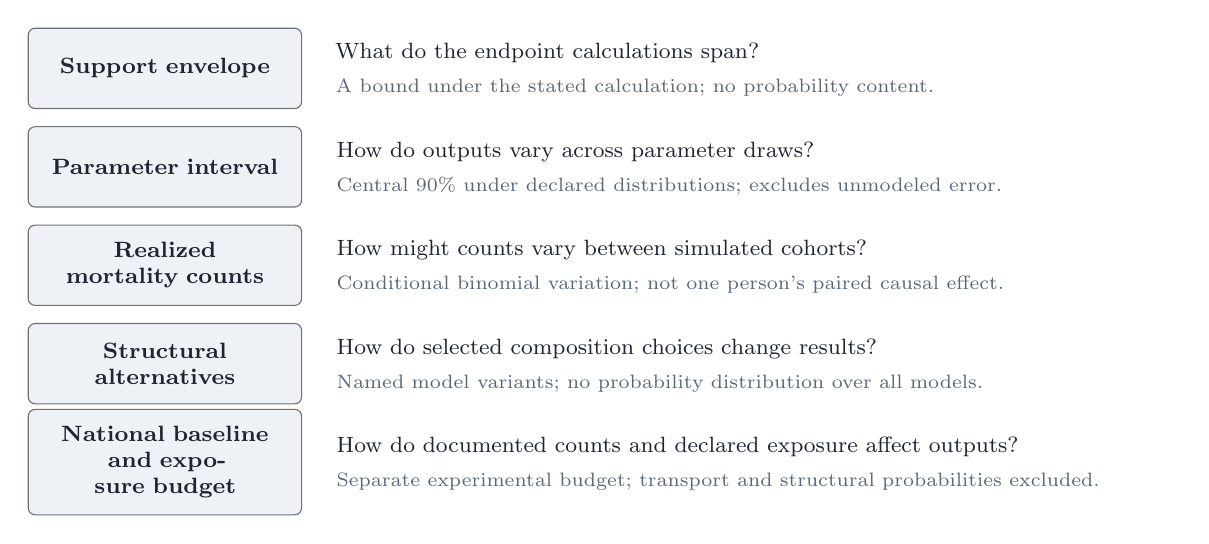
\begin{tikzpicture}
  \foreach \y/\rowtitle/\question/\explanation in {
    0/{Support envelope}/{What do the endpoint calculations span?}/{A bound under the stated calculation; no probability content.},
    -1.25/{Parameter interval}/{How do outputs vary across parameter draws?}/{Central 90\% under declared distributions; excludes unmodeled error.},
    -2.5/{Realized\\mortality counts}/{How might counts vary between simulated cohorts?}/{Conditional binomial variation; not one person's paired causal effect.},
    -3.75/{Structural\\alternatives}/{How do selected composition choices change results?}/{Named model variants; no probability distribution over all models.},
    -5/{National baseline\\and exposure budget}/{How do documented counts and declared exposure affect outputs?}/{Separate experimental budget; transport and structural probabilities excluded.}} {
    \node[fbox,fill=acc!9,anchor=west,text width=3.05cm,minimum height=1.02cm]
      at (0,\y) {\textbf{\rowtitle}};
    \node[anchor=west,align=left,text width=10.6cm,font=\footnotesize,text=ink]
      at (3.8,\y+0.19) {\question};
    \node[anchor=west,align=left,text width=10.6cm,font=\scriptsize,text=mut]
      at (3.8,\y-0.25) {\explanation};
  }
\end{tikzpicture}
\caption{Five distinct uncertainty summaries. They are not interchangeable
intervals. Default parameter draws hold baseline and exposure inputs fixed;
the separate national budget relaxes those assumptions. Study transport and
missing mechanisms remain outside both calculations.}
\label{fig:uncertainty}
\end{figure}


% @ref:paper-sampling
% Implementation: @link:code-distributions; @link:code-mc.
% Verification: @link:test-distributions.
% @tag:uncertainty
\subsection{Parameter sampling}
Latin hypercube sampling stratifies each parameter marginal
\cite{mckay1979}. Positive ratio units default to log-uniform sampling;
other undeclared marginals default to uniform bands. Rows can explicitly
select normal or lognormal shapes. The current normal-family sampler
clamps draws at the stated band limits. This is a bounded approximation
with endpoint mass, not sampling from a renormalized truncated-normal
density. The point is retained as the declared center when applicable.

Declared rank correlations can be imposed through an Iman--Conover
reordering \cite{iman1982}. The shipped table contains \CorrelationCount{} declared pairs linking
worker earnings with peak and sustained mortality. Their direction is
motivated by the shared recession context, but their moderate negative
magnitude is a declared assumption, not an extracted sampling covariance.
Unrolled copies of one intergenerational relationship share exactly one uncertainty draw, rather than independent copies. Sensitivity attribution groups those copies; independent-step analytic inference refuses chains that reuse the same relationship. Monte Carlo applies these pairs by default; analytic chains and standard
Sobol experiments retain their independence assumptions. Each Monte Carlo output records the seed, draw count, sampler,
and parameter version. Sample quantiles describe uncertainty conditional
on the specified distributions; they do not include all model error.

Scenario output separates three objects: endpoint support envelopes,
central 90\% parameter-only intervals, and simulated realized mortality
counts. For an integer cohort, let $S_0=(1-m)^Y$ and let $S_1$ be the
exposed survival product above. Conditional on each parameter draw,
\begin{equation}
 K_0\sim\operatorname{Binomial}(N,1-S_0),\qquad
 K_1\sim\operatorname{Binomial}(N,1-S_1),\qquad K_0\perp K_1.
\end{equation}
Then $E[K_1-K_0\mid\theta]=N(S_0-S_1)$. Both cohorts use the same
resolved county or national baseline. Their independent difference is a
reference-cohort contrast, not a paired individual causal effect.
Fractional worker equivalents and the legacy additive mortality method
do not receive this count simulation. Although the API calls it
``posterior-predictive,'' heterogeneous elicited parameter bands are not
a fitted joint Bayesian posterior; this is conditional predictive
simulation under the declared input distributions.

% @ref:paper-uncertainty-budget
% Implementation: @link:code-uncertainty-budget.
% Verification: @link:test-uncertainty-budget.
% @tag:uncertainty
\subsection{Separate baseline, exposure, and process budget}
The default scenario intervals above hold baseline and exposure inputs
fixed. The separate experimental \texttt{uncertainty} command relaxes
those restrictions for the national source-profile mortality scenario.
Documented baseline deaths $D_b$ and person-time $T_b$ must match the
verified rate and its sex, age, cause, calendar window, and geography.
With a Poisson likelihood and a declared Jeffreys rate prior, it samples
\begin{equation}
 \lambda\mid D_b,T_b\sim
 \operatorname{Gamma}(D_b+\tfrac12,\ \mathrm{rate}=T_b).
\end{equation}
Exposure is drawn from a caller-declared discrete uniform distribution
over integer bounds that bracket the reference cohort. That distribution
is a sensitivity assumption, not an inferred confidence distribution.
The calculation combines these inputs with parameter draws and retains
the original fixed-input reference. Expected-effect intervals and
independent-cohort binomial process contrasts are reported separately.

Baseline, exposure, and study parameters are assumed mutually independent,
while the two mortality persistence structures share each draw. Transport
error, probabilities over structures, missing mechanisms, age/time trends,
and uncertainty in child structure and earnings profiles remain excluded.
This national budget does not sample county posterior uncertainty or
support demographic-profile overrides. It is not a complete uncertainty
interval for an employer or individual and remains experimental.

% @ref:paper-inference
% Implementation: @link:code-inference.
% Verification: @link:test-inference.
% @tag:uncertainty
\subsection{Analytic moments and coverage}
For an independent level multiplier $X$, raw moments obey
$E[(VX)^k]=E[V^k]E[X^k]$. A direct step replaces the moments. For a gap
step with independent $T$ and $V$,
\begin{align}
 E[V'] &= 1-E[T]+E[T]E[V],\\
 E[(V')^2] &= 1-2E[T]+E[T^2]
 +2(E[T]-E[T^2])E[V]+E[T^2]E[V^2].
\end{align}
The implementation also propagates third moments for supported
marginals. It uses them for skewness and Cornish--Fisher quantile
approximations. Exact moments do not make those approximate quantiles
exact. Unsupported distribution cases are refused. The identities also
require that each new multiplier be independent of the accumulated
quantity; reuse of a parameter can violate that condition.

Monte Carlo comparisons check the analytic calculations. Coverage closure
experiments draw synthetic truths under the declared model and measure
whether independently built intervals cover them. These tests assess
interval machinery under its own assumptions. They cannot establish
coverage for real-world events. Correlation stress experiments similarly
price a hypothetical dependence choice without treating it as evidence.

% @ref:paper-sensitivity
% Method: @link:doc-result-sensitivity.
% Implementation: @link:code-sensitivity; @link:code-knobs; @link:code-variants.
% Verification: @link:test-sensitivity-scoring.
% @tag:uncertainty
\subsection{Sensitivity, sweeps, and structural variants}
The sensitivity interface estimates first-order and total Sobol indices
using a Saltelli-style design \cite{sobol2001,saltelli2002}. Seed replicates
report design variation; that spread is not a confidence interval on the
true index. Standard variance attribution assumes independent inputs.
A place adjustment can make the mobility coefficient contribute to
child-line sensitivity even though it has no effect at the national
reference.

A separate correlated-block option groups all connected dependent
parameters and swaps each joint block between independently seeded
designs. It estimates attribution to independent blocks, not to
individual dependent coefficients. Reusing a fixed copula rank template
across the two designs invalidates that experiment; the current repair
tests it against an additive model with known block variance shares.

A sweep pins one parameter inside its cited band and recomputes scenario
counts. A value-of-information experiment narrows each parameter band
around its point and compares output-band widths on a common seed.
This is a precision-priority heuristic, not an expected utility
calculation or a prediction of what a new study will find. Experiments
carry a version marker and do not overwrite the published parameter set.
Structural ensembles report named alternatives for gap additivity,
transmission decay, finite-change log elasticity, and closure selection.
Scenario mortality additionally reports the persistence comparison above.
Their spread represents
selected assumptions, not a probability distribution over all possible
models.

The policy comparator subtracts caller-supplied exposure scenarios.
It reports a conservative difference of support envelopes, with exact
cancellation for identical cases. Shared-draw paired contrasts are a
future improvement; the current envelope is not a probabilistic policy
effect interval and does not identify a policy-to-exposure bridge.

% @ref:paper-synthesis
% Method: @link:doc-pool-readiness-0-4.
% Implementation: @link:code-synthesis; @link:code-county-rates.
% Verification: @link:test-synthesis.
% @tag:evidence
\subsection{Evidence synthesis and county likelihoods}
The optional synthesis module implements DerSimonian--Laird heterogeneity
estimation and inverse-variance random-effects pooling only after exact
link, scale, population, and horizon checks, with declared treatment,
comparison, outcome, and overlap metadata retained for review. Its intervals use a plug-in normal approximation;
uncertainty in the estimated between-study variance is not propagated.
Few-study prediction intervals can be unreliable \cite{cochraneMeta}.
Matching scale strings alone does not enforce compatible follow-up,
population, design, or independent samples. Metadata review remains
necessary, and these outputs are not automatically admitted as parameters.

The standalone county module uses
$D\mid\lambda\sim\operatorname{Poisson}(T\lambda)$ with a gamma prior,
where $T$ is compatible person-time, and reports the constant-hazard
conversion $1-\exp(-\lambda)$ separately from the rate likelihood. It
requires national-prior outcome, population, and window metadata to match
the county observation. The county module is not integrated into scenario
baseline uncertainty.

% @ref:paper-validation
% Method: @link:doc-scenario-evidence-protocol.
% Implementation: @link:code-validate; @link:code-scoring.
% Verification: @link:test-validate.
% @tag:validation
\section{Validation results}
% @ref:paper-v0
% Implementation: @link:code-validate.
% Verification: @link:test-validate.
% @tag:validation
\subsection{V0: internal consistency}
The direct child estimate is \VzeroDirect{}, while the worker-shock path
composed with intergenerational transmission is \VzeroComposed{}.
Their bands overlap. This checks compatibility between two modeled paths;
it does not provide an independent validation of their causal claims.

% @ref:paper-v1-units
% Implementation: @link:code-validate.
% Verification: @link:test-retrodict.
% Related: @link:figure-unit-checks.
% @tag:validation
\subsection{V1: China-shock unit scorecard}
Figure~\ref{fig:unit-checks} plots the unit comparisons. Exact values are
retained in Appendix~\ref{app:scorecards}.
The unit scorecard uses the exposure bridge and measured coefficients
transcribed from Autor, Dorn, and Hanson \cite{autor2019}. The bridge
maps an import shock into manufacturing displacement. The downstream
mortality path uses a separate study \cite{sullivan2009}, but comparing
it with a commuting-zone male--female mortality differential requires
strong population and outcome-transfer assumptions.


\begin{figure}[t]
\centering
\scorelegend\par\medskip
\textbf{A. Mortality: modeled bands and measured targets}\par\smallskip
\input{generated/mortality_plot_limits.tex}
\begin{tikzpicture}[trim axis left,trim axis right]
  \begin{axis}[score, height=3.0cm, xmin=\PlotMin, xmax=\PlotMax, ymax=2.55,
    xtick distance=\PlotStep, ytick={0,1,2},
    yticklabels={All adults,All male,{All male, age matched}},
    xlabel={Excess deaths per 100,000 adults per unit shock}]
    \scoreplot{generated/mortality_plot.dat}
  \end{axis}
\end{tikzpicture}\par\bigskip
\textbf{B. Divorce path: both windows fall short of the stock change}\par\smallskip
\input{generated/divorce_plot_limits.tex}
\begin{tikzpicture}[trim axis left,trim axis right]
  \begin{axis}[score, height=2.4cm, xmin=\PlotMin, xmax=\PlotMax, ymax=1.55,
    xtick distance=\PlotStep, ytick={0,1}, yticklabels={5-year window,10-year window},
    xlabel={Percentage points of women per unit shock}]
    \scoreplot{generated/divorce_plot.dat}
  \end{axis}
\end{tikzpicture}
\caption{China-shock unit checks generated from the current engine.
Blue lines are model bands, not a common confidence level; amber diamonds
are measured point targets without their sampling intervals. Panel A compares
modeled mortality with a male--female differential; panel B compares divorce
with a broader family-status stock change. These target mismatches limit both
comparisons. Numerical values appear in Appendix~\ref{app:scorecards}.}
\label{fig:unit-checks}
\end{figure}


\input{generated/mortality_summary}
A measured
confidence interval and a modeled parameter band answer different
questions; overlap is not proof of validity. The full JSON scorecard
also reports whether the modeled point lies inside the measured interval.
Age matching does not remove the distinction between an absolute
mortality level and a sex differential, nor the transfer from
high-seniority displaced workers to a broader exposed population.




The divorce path uses independent displacement studies
\cite{rege2007,charles2004} and a marriage baseline. Its point estimates
undershoot the observed family-status stock change at both windows.
That stock includes widowhood and separation; divorce incidence alone
cannot reproduce all its margins. Remarriage is a candidate missing
mechanism, not an extracted explanation. Several additional target
outcomes are withheld because the implemented evidence path would reuse
the target coefficient rather than provide an independent comparison.

% @ref:paper-v1-panel
% Implementation: @link:code-validate; @link:code-scoring.
% Verification: @link:test-panel.
% Related: @link:figure-panel-checks.
% @tag:validation
\subsection{V1: commuting-zone contrasts and scoring}
Figure~\ref{fig:panel-checks} plots the panel contrasts on separate axes
for family status and earnings.
The deposited panel extract contains \PanelCount{} commuting-zone-period
rows. Comparisons demean exposure and outcomes within period before
contrasting high- and low-shock terciles. Pooling without that adjustment
confounds period differences and changes the sign of the family-status
comparison. The tests retain this failure mode.


% @ref:figure-panel-checks
% Verification: @link:test-panel.
% Related: @link:paper-v1-panel; @link:paper-build-tables.
% @tag:validation
\begin{figure}[t]
\centering
\scorelegend\par\medskip
\textbf{A. Family status: both measured contrasts lie in the model bands}\par\smallskip
\input{generated/panel_divorce_plot_limits.tex}
\begin{tikzpicture}[trim axis left,trim axis right]
  \begin{axis}[score, height=2.4cm, xmin=\PlotMin, xmax=\PlotMax, ymax=1.55,
    xtick distance=\PlotStep, ytick={0,1}, yticklabels={Pooled,Male shock},
    xlabel={High-minus-low-shock contrast (percentage points)}]
    \scoreplot{generated/panel_divorce_plot.dat}
  \end{axis}
\end{tikzpicture}\par\bigskip
\textbf{B. Earnings: adding spillover reduces the miss but does not close it}\par\smallskip
\input{generated/panel_earnings_plot_limits.tex}
\begin{tikzpicture}[trim axis left,trim axis right]
  \begin{axis}[score, height=2.4cm, xmin=\PlotMin, xmax=\PlotMax, ymax=1.55,
    xtick distance=\PlotStep, ytick={0,1},
    yticklabels={Direct,{With spillover}},
    xlabel={High-minus-low-shock contrast (USD)}]
    \scoreplot{generated/panel_earnings_plot.dat}
  \end{axis}
\end{tikzpicture}
\caption{Within-period-demeaned commuting-zone contrasts from
\PanelCount{} zone-period rows. Model points and bands come from the same
generated scorecard as the tables. Measured diamonds omit sampling uncertainty;
point coverage alone is not validation. The wage-spillover addition followed
the original miss and is not an independent held-out success. Axes retain the
outcomes' different units.}
\label{fig:panel-checks}
\end{figure}


The family-status contrasts are covered. Direct worker earnings losses
alone substantially underpredict the observed lower-quartile earnings
change. Adding the non-displaced wage response \cite{adh2013} reduces
that gap but does not eliminate it. The earlier direct-only miss remains
beside the composed result. The spillover extension was motivated by
the observed miss; it is a diagnostic revision, not a fresh held-out
success. Shared China-shock evidence further limits independence.

\input{generated/slope}
CRPS summarizes distance between a predictive distribution and an observed
point; PIT locates that point within the distribution
\cite{hersbach2000}. Scoring against a published coefficient treats its
point estimate as the target and does not integrate its measurement
uncertainty. The upper-tail PIT and earnings residual show why selected
tercile coverage should not be described as overall model validation.

% @ref:paper-independent-validation
% Method: @link:doc-scenario-evidence-protocol.
% Implementation: @link:code-forecast-registry.
% Verification: @link:test-v2-backtest; @link:test-forecast-fsm.
% @tag:validation
\subsection{V2 and V3: incomplete validation}
Independent-event protocols exist for NAFTA, the auto crisis, and BRAC.
Their scorecards are blocked on event-specific exposure bridges or
measured outcome inputs. A tariff change cannot inherit an
import-penetration displacement bridge merely because both concern
trade. Descriptive employment loss does not supply a quasi-experimental
measured outcome. No completed V2 event score is claimed here.

Prospective registration and scoring checks are implemented, but no
real event has yet been registered. It requires forecasts fixed
before outcomes are available, a declared exposure and time horizon,
and a scoring rule fixed before evaluation. No prospective result is
reported. Unit and panel V1 results are the current external checks.

% @ref:paper-descriptive-checks
% Method: @link:doc-baseline-transition-r2-2026-09-14.
% Implementation: @link:script-build-displaced-cohort; @link:script-evaluate-followthrough.
% @tag:data
\subsection{Descriptive cohort and baseline checks}
The reproducible CPS January-2024 reference describes known-year
2021--2023 displacements with lost-job tenure of at least three years,
with a separate six-year-tenure subset. Survey weights reproduce the
rounded published BLS total. Age and household composition are measured
at interview and cannot silently stand in for historical event-age
characteristics. Neither cohort identifies H-1B-specific displacement.
The held-out SIPP checks compare baseline transition probabilities;
they do not validate displacement effects or household recovery.
\input{generated/followthrough}
These archived results are retained in
\nolinkurl{validation/followthrough_evaluation_expanded_20261014.json}.
Its compatible-pooling refusals preserve population, horizon, scale, and
overlap differences rather than manufacture independent study counts.
The source-selection and evaluation protocol in
\nolinkurl{docs/SCENARIO_EVIDENCE_PROTOCOL.md} records a locally frozen
research round, not retrospective preregistration or an independently
timestamped prospective forecast. No new matched independent event score
is established by these software and baseline-data checks.

\FloatBarrier
% @ref:paper-limitations
% Method: @link:doc-model-card; @link:doc-citing.
% @tag:methods
\section{Limitations}
The model conditions on displacement and does not identify who was
displaced or why. An upstream employer exposure can therefore be more
uncertain than the downstream parameter band suggests. The entity
adapter checks arithmetic and provenance fields, not the factual or
causal validity of the supplied records.

Studies differ in country, age, sex, tenure, and measurement window.
Transporting them across populations is a substantive assumption.
Default mortality uses a constant baseline and the five-phase source-offset
profile described above. The separate age-stratum projection advances
age-band baselines under a different, constant source-window response
assumption; neither models individual risk factors or resolves source-to-target
transport. Lifetime earnings conversion uses a synthetic
cross-sectional profile. Local employment multipliers omit migration
and equilibrium adjustment. These choices can affect magnitudes even
when arithmetic and citations are correct.

Transmission across distant generations is weakly identified. Parallel
family pathways may overlap, place adjustments transfer a rank effect to
an earnings scale, and repeated place steps can magnify the adjustment.
None of these is resolved by collecting more Monte Carlo draws.

The current bands use heterogeneous evidence conventions and simplified
marginal shapes. Only the declared correlation pairs enter Monte Carlo; other dependencies
remain unmodeled. Place measurements and baseline estimates are generally
fixed in default scenario sampling. The separate national uncertainty
budget includes documented baseline-count and declared exposure
distributions under additional assumptions. Household intervals and
county posterior sampling remain unavailable. Structural ensembles cover only
selected alternatives. Internal coverage tests therefore validate
machinery, while V1 exposes economic and measurement discrepancies.
There is no basis for treating the output as a complete uncertainty
interval for an individual, employer, or community.

The repository also records refused and contested links. It does not
encode a positive immigration-to-crime effect from a pooled literature
that does not support one \cite{ousey2018,butcher1998}. Observational
findings may supply cross-checks without setting a causal point.
Named competing specifications must remain visible rather than being
averaged into a preferred headline.

% @ref:paper-development
% Method: @link:doc-life-course-research-plan; @link:doc-causal-graph-plan.
% @tag:model
\section{Prioritized development}
The next work should evaluate the experimental capabilities now implemented.
The national baseline/exposure budget, age-stratum mortality projection,
child present values, and household comparison each retain specific
applicability and uncertainty limits. Extend baseline sampling to compatible
county inputs, quantify target-population transport, and assess the
constant-hazard conversion. Resolve the place counterfactual before adding
further place-driven descendants. Review effect scale, intervention,
mediator versus total effect, source population, and window metadata;
compatible units alone do not establish causal composability.

Expand compatible independent study pools with overlap and window checks
and small-sample synthesis sensitivity. Preserve null, protective, and
conflicting effects. Broaden age/sex/tenure response support only with source
estimates; adding baseline strata alone does not identify effect modifiers.
Estimate survey-design uncertainty and assess longer-run stability of the
SIPP transition cells. For the already separate manufacturing and high-tech
job multipliers, test whether expansion effects transfer symmetrically to
displacement.

Validation should prioritize one completed independent event before
expanding the graph: freeze a matched exposure bridge, geography,
population, outcome window, and observation model, then report every
scored outcome. Register one prospective forecast with an independent
timestamp. Numerical tests should include null-intervention invariance,
same-place counterfactual cancellation, independently seeded sampling
designs, and known analytic variance shares. These checks complement
the existing property tests; passing code tests cannot repair an
unidentified causal bridge.

% @ref:paper-research-program
% Method: @link:doc-life-course-research-plan.
% Related: @link:figure-future.
% @tag:model
\subsection{A person-and-place research program}
Figure~\ref{fig:future} summarizes the implemented household prototype
and the research gates that still precede public use.
\begin{figure}[t]
\centering
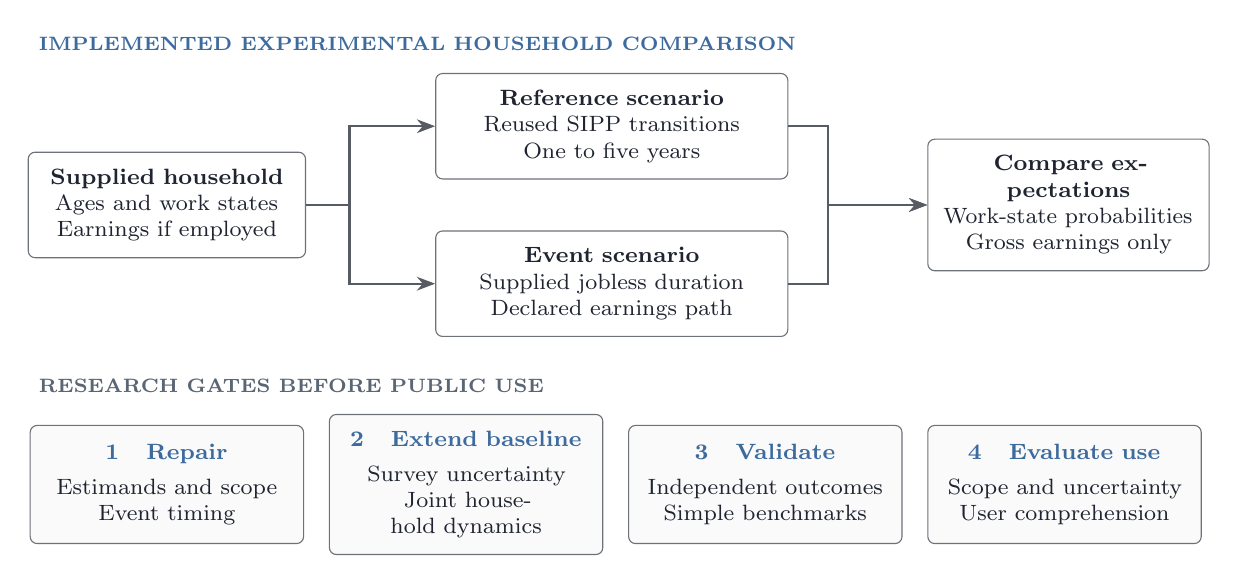
\begin{tikzpicture}
  \node[anchor=west,font=\scriptsize\bfseries,text=acc] at (0,1.05)
    {IMPLEMENTED EXPERIMENTAL HOUSEHOLD COMPARISON};
  \node[fbox,text width=3.1cm,minimum height=1.25cm] (profile) at (1.75,-1.0)
    {\textbf{Supplied household}\\Ages and work states\\Earnings if employed};
  \node[fbox,text width=4.05cm,minimum height=1.15cm] (reference) at (7.4,0)
    {\textbf{Reference scenario}\\Reused SIPP transitions\\One to five years};
  \node[fbox,text width=4.05cm,minimum height=1.15cm] (event) at (7.4,-2.0)
    {\textbf{Event scenario}\\Supplied jobless duration\\Declared earnings path};
  \node[fbox,text width=3.15cm,minimum height=1.4cm] (compare) at (13.2,-1.0)
    {\textbf{Compare expectations}\\Work-state probabilities\\Gross earnings only};
  \draw[flow] (profile.east) -- ++(0.55,0) |- (reference.west);
  \draw[flow] (profile.east) -- ++(0.55,0) |- (event.west);
  \draw[flow] (reference.east) -- ++(0.5,0) |- (compare.west);
  \draw[flow] (event.east) -- ++(0.5,0) |- (compare.west);
  \node[anchor=west,font=\scriptsize\bfseries,text=mut] at (0,-3.3)
    {RESEARCH GATES BEFORE PUBLIC USE};
  \foreach \x/\num/\heading/\detail in {
    1.75/1/{Repair}/{Estimands and scope\\Event timing},
    5.55/2/{Extend baseline}/{Survey uncertainty\\Joint household dynamics},
    9.35/3/{Validate}/{Independent outcomes\\Simple benchmarks},
    13.15/4/{Evaluate use}/{Scope and uncertainty\\User comprehension}} {
    \node[fbox,fill=black!2,text width=3.05cm,minimum height=1.5cm] at (\x,-4.55)
      {\textcolor{acc}{\textbf{\num\quad\heading}}\\[3pt]\detail};
  }
\end{tikzpicture}
\caption{The implemented household prototype and its remaining release gates.
Both scenarios start from the same supplied household. Observed transitions
and supplied unemployment duration define conditional expectations, not an
identified causal recovery path. Joint household dynamics, further events,
community feedback, and longer horizons require additional evidence and validation.}
\label{fig:future}
\end{figure}


The longer-term target is a distribution of possible outcomes conditional
on a supplied profile and specified event, with an explicit reference
scenario. It requires a baseline model of how employment, income, health,
household relationships, and location evolve without that event. Baseline
transitions may be estimated from documented longitudinal data; their
predictive associations must be distinguished from identified causal
intervention effects and from declared structural assumptions.

Personalization should distinguish characteristics that change baseline
risks from those supported as effect modifiers. A location field does not
establish a county-specific treatment effect. Linked household members,
children's ages, shared resources, and event histories are necessary for
family consequences. Community spillovers require an appropriate
population model; summing person-level effects does not identify every
regional response. Event definitions must include onset, duration, dose,
comparison condition, and ordering. Unsupported interactions remain
unresolved even when each event has an individual effect estimate.

The implemented five-year synthetic household demonstration compares
employment probabilities and gross earnings with and without a supplied
displacement duration. The next research step is to evaluate that restricted
comparison against simple benchmarks and independently matched outcomes,
then extend linked family dynamics only where justified. A protective
intervention can follow when independently supported. Shared random draws
can improve sampled comparison precision; the current household prototype
instead calculates marginal expectations exactly. Neither identifies one
person's joint potential outcomes. A full life-course simulator and public
applicability are not established. Milestones and acceptance criteria are recorded in
\nolinkurl{docs/LIFE_COURSE_RESEARCH_PLAN.md}.

% @ref:paper-calculator
% Method: @link:doc-calculator; @link:doc-website-experience-plan.
% Implementation: @link:calculator-math.
% Verification: @link:test-calculator.
% @tag:calculator
\subsection{Public calculator as a research interface}
An eventual website should make the profile, event, comparison, outcome
unit, time horizon, and evidence applicability visible together. It should
show absolute outcomes and scenario differences, distinguish uncertainty
about the model from variation among simulated lives, and separate missing
evidence from a supported null effect. Information should unfold from a
short comparison to trajectories, assumptions, and study receipts, without
requiring the visitor to understand a graph before using the calculator.
Neutral scenario colors, legible charts, accessible controls, and clear
unsupported-result states are part of scientific communication.

Initial public use should be restricted to evaluated scenarios and supported
profiles. A synthetic example can demonstrate interaction before those
capabilities are ready, but must be labeled as illustrative. Usability
evaluation should measure whether visitors understand the comparison and
its limits, rather than treating visual polish or expressed trust as
evidence of comprehension. The separate product plan,
\nolinkurl{docs/WEBSITE_EXPERIENCE_PLAN.md}, specifies the intended journey,
visual direction, explanation patterns, and release criteria; it is a
design proposal, not a description of a deployed service.

% @ref:paper-reproducibility
% Method: @link:doc-paper; @link:doc-consumer-fixtures-0-4.
% Implementation: @link:script-build-methods-html.
% Related: @link:paper-build-tables.
% @tag:methods
\section{Reproducibility and availability}
The model and paper source are provided under the repository's MIT
license. Run the tests, \texttt{downstream audit}, and
\texttt{downstream validate} to inspect implementation and evidence
checks. Sampling commands record their seeds and draw counts. Parameter
exports carry a version; the paper also records a content digest because
parameter version alone does not identify engine code changes. The
September 10 review repaired county predictive-baseline consistency,
disconnected custom chains, ignored chain starting values, and the
fixed copula seed used in sensitivity designs. Correlated Monte Carlo
results can consequently change at the same historical user seed.

Running \texttt{make -C paper} regenerates tables and chart data, builds the PDF, and
writes \nolinkurl{paper/generated/results.json}. This JSON contains the
full validation output and the source SHA-256. The appendix
and coverage interpretation use the same live scorecard; reference
mortality persistence values are generated from the scenario code. The
archived follow-through evaluation is separately labeled in the JSON.
The generated appendix preserves parameter points, bands, tiers, and citation keys. Population
scope, distribution declarations, and extraction notes remain in the
underlying CSV files. Source content digest for this build begins
\texttt{\SourceDigest}. Generated numerical results are not manually
copied into the prose. Vector diagrams and charts use the same restrained
palette throughout. Model bands and measured points differ in both color
and marker shape. Chart coordinates retain the engine's unrounded values;
the tables provide compact rounded readings. The digest manifest includes engine code, parameter and validation CSV, JSON and XML inputs, and build scripts/configuration. A semantic HTML companion at \nolinkurl{docs/methods.html} supplies readable text, scoped tables, baseline qualifications and a complete CSV download. The PDF remains an untagged publication artifact; the HTML companion is the accessible reading path.

\clearpage
\appendix
% @ref:paper-scorecards
% Implementation: @link:code-validate.
% Verification: @link:test-paper-tables.
% Related: @link:paper-build-tables.
% @tag:validation
\section{Numerical validation scorecards}\label{app:scorecards}
These tables retain the exact comparison structure behind
Figures~\ref{fig:unit-checks} and~\ref{fig:panel-checks}.
Values are rounded to four decimal places; chart coordinates use the
unrounded engine output. ``Covered'' means only that the measured point
lies in the model band, not that the model is causally validated.

\begin{table}[H]
\centering\small
\caption{Mortality per 100,000 adults per unit shock. Coverage asks whether
 the measured point lies in the modeled band.}
\begin{tabular}{lrrc}
\toprule Variant & Model point [band] & Measured & Covered? \\ \midrule
\tableinput{generated/mortality.tex}
\bottomrule
\end{tabular}
\end{table}

\begin{table}[H]
\centering\small
\caption{Unit divorce-path predictions in percentage points of women,
compared with the measured family-status stock change.}
\begin{tabular}{rrr}
\toprule Window (years) & Model point [band] & Measured \\ \midrule
\tableinput{generated/divorce.tex}
\bottomrule
\end{tabular}
\end{table}

\begin{table}[H]
\centering\small
\caption{Within-period-demeaned panel contrasts. Coverage uses the
measured contrast as a point target.}
\begin{tabular}{lrrc}
\toprule Outcome & Model point [band] & Measured & Covered? \\ \midrule
\tableinput{generated/panel.tex}
\bottomrule
\end{tabular}
\end{table}

\clearpage
% @ref:paper-parameter-inventory
% Method: @link:doc-citing; @link:doc-attribution.
% Implementation: @link:code-params.
% @tag:evidence
\section{Current parameter set}\label{app:parameters}
The table is an inventory, not a claim that every row belongs to one
composable causal chain. Values use each destination node's declared
unit in \nolinkurl{params/nodes.csv}. Different rows cannot be compared
as if their numbers shared a scale. Parameter values below are rounded to
four decimal places; the source CSV retains full precision and identifiers. Readable relationship labels are used here to prevent identifier fragments. A semantic HTML companion is generated at \nolinkurl{docs/methods.html}.
\begingroup\footnotesize
\setlength{\tabcolsep}{4pt}
\begin{longtable}{>{\raggedright\arraybackslash}p{2.65in}>{\raggedright\arraybackslash}p{1.35in}>{\raggedright\arraybackslash}p{0.75in}>{\raggedright\arraybackslash}p{0.9in}}
\caption{Generated parameter inventory, \ParameterVersion.}\\
\toprule Relationship & Point [band] & Tier & Sources \\ \midrule\endfirsthead
\toprule Relationship & Point [band] & Tier & Sources \\ \midrule\endhead
\bottomrule\endfoot
\tableinput{generated/parameters.tex}
\end{longtable}
\endgroup
\bibliographystyle{plain}
\bibliography{generated/references,review_references}
\end{document}
